\chapter{工作结论}
\label{chap:5}

本次作业从第一章对用线图绘制介面,从而确定整个系统的大致功能需求,另外从团队角度出发并考量整体成员的能力,研究所需要开发的技术跟工具,同时进行测试工作的分配。过程中讨论与分析,如何辨识学生的上课状况是否疲倦的主体原因,并找出本作业在定义流程的理论依据与文献,此作业主要贡献在于,面对深度学习与计算机视觉等研究工作下,提供一个相对稳定的 Web 服务的展示环境。同时团队也探讨整体的开发流程与技术跟研究工作的整合,因此本作业将在未来展望进行说明。

\section{未来展望}

本作业在进行开发与测试过程中讨论的三个后续发展的可用工作,分别为第一节的实际设计工具 Figma ,第二节为需要改善的团队流程,最后则是快速部属的虚拟化应用。

\subsection{实际设计}

本作业在实际用线图规划出大致的功能后,实际上要开始设计桌面应用与未来行动的使用者介面,而当中使用可以多人协作的平台 Figma,毕竟当需求厘清时,要同时考量到前端工程、测试人员、设计师广泛的讨论,当中很多功能的外观必须由此确定。

\begin{figure}[htb]
\centering 
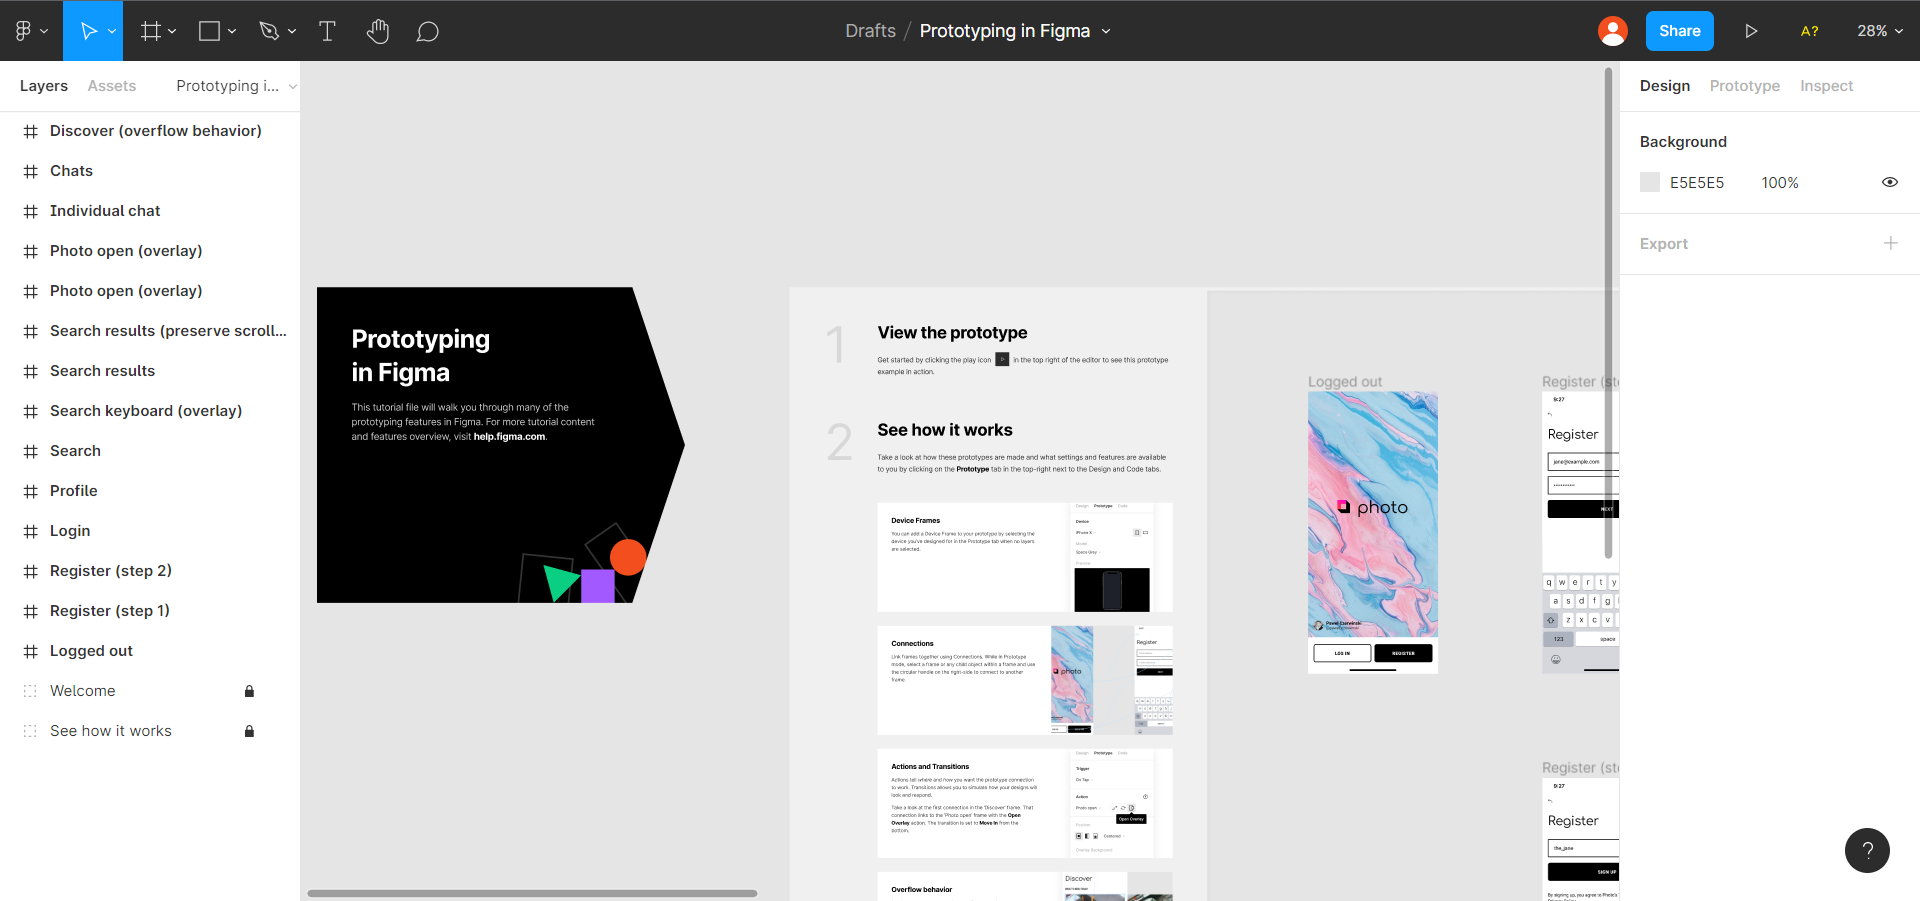
\includegraphics[width=0.80\textwidth]{img/ch5m1.png} 
\caption{Figma 平台画面}
\label{Test}
\end{figure}

\subsection{导入团队开发流程}

多人与多团队合作的状况下,不同于单人独立作业的状况,基本上在实际整个专案开发时,master 为主要的分支,一般更动会建立开发的分支, master 的更动是稳定的版本,而团队成员则是根据开发的分支 develop,再建立分支进行修正与添加新功能,完成后提出 Pull Request ,审核后合并进 develop ,其后再整合进 master ,使其系统上线。

\begin{figure}[htb]
\centering 
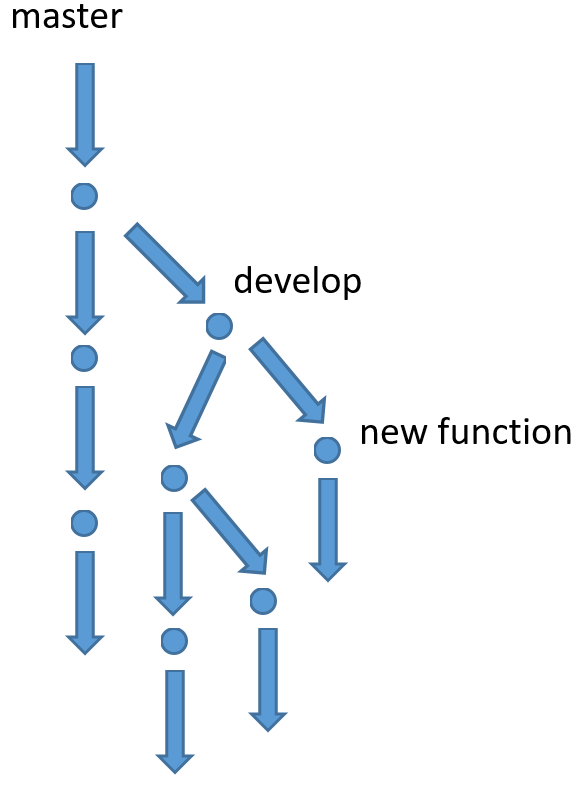
\includegraphics[width=0.80\textwidth]{img/ch5m2.png} 
\caption{Git 版本与发布概念}
\label{Test}
\end{figure}

\subsection{快速部属的工作流程}

在此主要讨论的是在持续部署与测试的考量,本次作业线上开发的过程面对大量的不同平台设备所遭遇到的环境部属问题,因此讨论 Docker 的运用,其 Docker 在开发与运维的领域中具有极大的吸引力,因为它能保持跨环境的一致性。

因为开发与发布的生命周期中,不同的环境具有细微的不同,这些差异可能是由于不同安装的版本与不同的套件和依赖关系所引起。然而 Docker 可以通过确保从开发到产品发布整个过程环境的一致性来解决这个问题。因为 Docker 容器通过相关配置,保持容器内部所有的配置和依赖关系始终不变。最终可以在开发到产品发布的整个过程中使用相同的容器来确保没有任何差异或者人工干预,加速团队的工作流程。另外以 python3.7 为基础镜像构建的 Dockerfile 编写档案如下所示。

\begin{figure}[htb]
\centering 
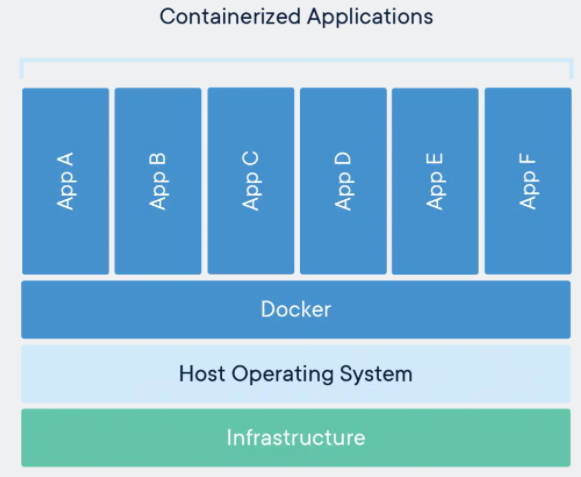
\includegraphics[width=0.80\textwidth]{img/ch5m3.png} 
\caption{Docker 概念}
\label{Test}
\end{figure}


\begin{Verbatim}
# 以 python3.7 为基础镜像构建
FROM python:3.7
# 安装nginx与supervisor
RUN apt-get update && apt-get install -y nginx supervisor
# 安装gevent与gunicorn
RUN pip install gunicorn pipenv
# 解决输出可能的中文乱码
ENV PYTHONIOENCODING=utf-8

# 创建并设置工作目录
WORKDIR /project/flask-app
# 拷贝包文件到工作目录
COPY Pipfile* /project/flask-app/
# 安装包
RUN pipenv install --system

# nginx配置相关
# 删除默认的有效配置,sites-enabled 目录下的配置文件才能够真正被用户访问
RUN rm /etc/nginx/sites-enabled/default
# 将配置文件链接到sites-available目录
RUN ln -s /etc/nginx/sites-available/nginx.conf /etc/nginx/sites-enabled/nginx.conf
# 添加自定义CMD时,添加此命令到nginx全局配置中保证容器可以跟踪到进程,防止容器退出
RUN echo "daemon off;" >> /etc/nginx/nginx.conf

# supervisord配置相关
RUN mkdir -p /var/log/supervisor
# 指定容器运行启动命令
CMD ["/bin/bash"]
\end{Verbatim}
